\section{Introduction}

In recent years neural methods for Natural Language Processing (NLP) have consistently and repeatedly improved the state-of-the-art in a wide variety of NLP tasks such as parsing, PoS-tagging, named entity recognition, machine translation, text classification and reading comprehension among others. Probably the main contributing factor in this steady improvement for NLP models is the raise in usage of \emph{transfer learning} techniques in the field. These methods normally consist of taking a pre-trained model and reusing it, with little to no retraining, to solve a different task from the original one it was intended to solve; in other words, one \emph{transfers} the \emph{knowledge} from one task to another.

Most of the transfer learning done in NLP nowadays is done in an unsupervised manner, that is, it normally consist of a  \emph{language model} that is fed unannotated plain text in a particular language; so that it \emph{extracts} or \emph{learns} the basic \emph{features} and patterns of the given language, the model is subsequently used on top of an specialised architecture designed to tackle a particular NLP task. Probably the best known example of this type of model are \emph{word embeddings} which consist of real-valued vector representations that are trained for each word on a given corpus. Some notorious examples of word embeddings are word2vec \citep{mikolov-etal-2013-distributed}, GloVe \citep{pennington-etal-2014-glove} and \mbox{fastText} \citep{mikolov-etal-2018-advances}. All these models are \emph{context-free}, meaning that a given word has one single vector representation that is independent of context, thus for a polysemous word like Washington, one would have one single representation that is reused for the city, the state and the US president.

In order to overcome the problem of polysemy, \emph{contextual} models have recently appeared. Most notably ELMo \citep{peters-etal-2018-deep} which produces deep contextualised word representations out of the internal states of a deep bidirectional language model in order to model word use and how the usage varies across linguistic contexts. ELMo still needs to be used alongside a specialised architecture for each given downstream task, but newer architectures that can be fine-tuned have also appear. For these, the model is first fed unannotated data, and is then fine-tuned with annotated data to a particular downstream task without relying on any other architecture. The most remarkable examples of this type of model are GPT-1, GPT-2 \citep{radford-etal-2018-improving,radford-etal-2019-language}, BERT \citep{devlin-etal-2019-bert} and XLNet \citep{yang-etal-2019-xlnet}; the latter being the current state-of-the-art for multiple downstream tasks. All of these models are different arrangements of the Transformer architecture \citep{vaswani-etal-2017-attention} trained with different datasets, except for XLNet which is an instance of the Transformer-XL \citep{dai-etal-2019-transformer}.

Even though these models have clear advantages, their main drawback is the amount of data that is needed to train them in order to obtain a functional and efficient model. For the first English version of word2vec, \citet{mikolov-etal-2013-distributed} used a one billion word dataset consisting of various news articles. Later \citet{al-rfou-etal-2013-polyglot} and then \citet{bojanowski-etal-2017-enriching} used the plain text from Wikipedia to train distributions of word2vec and fastText respectively, for languages other than English. Now, the problem of obtaining large quantities of data aggravates even more for contextual models, as they normally need multiple instances of a given word in order to capture all its different uses and in order to avoid overfitting due to the large quantity of hyperparameters that these models have. \citet{peters-etal-2018-deep} for example use a 5.5 billion token\footnote{Punctuation marks are counted as tokens.} dataset comprised of crawled news articles plus the English Wikipedia in order to train ELMo, \citet{devlin-etal-2019-bert} use a 3.3 billion word\footnote{Space sparated tokens.} corpus made by merging the English Wikipedia with the BooksCorpus \citep{zhu-etal-2015-aligning}, and \citet{radford-etal-2019-language} use a 40GB English corpus created by scraping outbound links from Reddit.\footnote{\url{https://www.reddit.com/}}

While Wikipedia is freely available, and multiple pipelines exist\footnote{\url{https://github.com/attardi/wikiextractor}}\textsuperscript{,}\footnote{\url{https://github.com/hghodrati/wikifil}} to extract plain text from it, some of the bigger corpora mentioned above are not made available by the authors either due to copyright issues or probably because of the infrastructure needed to serve and distribute such big corpora. Moreover the vast majority of both these models and the corpora they are trained with are in English, meaning that the availability of high quality NLP for other languages, specially for low-resource languages, is rather limited.

To address this problem, we choose Common Crawl\footnote{\url{http://commoncrawl.org/}}, which is a 20TB mutilingual free to use corpus composed of crawled websites from the internet, and we propose a highly parallel multithreaded asynchronous pipeline that applies well-known concurrency patterns, to clean and classify by language the whole Common Crawl corpus to a point where it is usable for Machine Learning and in particular for neural NLP applications. We optimise the pipeline so that the process can be completed in a sensible amount of time even in infrastructures where Input/Output (I/O) speeds become the main bottleneck.

Knowing that even running our pipeline will not always be feasible, we also commit to publishing our own version of a classified by language, filtered and ready to use Common Crawl corpus upon publication of this article. We will set up an easy to use interface so that people can download a manageable amount of data on a desired target language.

\section{Related Work}

Common Crawl has already been successfully used to train language models, even multilingual ones. The most notable example in probably fastText which was first trained for English using Common Crawl \citep{mikolov-etal-2018-advances} and then for other 157 different languages \citep{grave-etal-2018-learning}. In fact \citet{grave-etal-2018-learning} proposed a pipeline to filter, clean and classify Common Crawl, which we shall call the ``fastText pre-processing pipeline.'' They used the fastText linear classifier \citep{joulin-etal-2016-fasttext, joulin-etal-2017-bag} to classify each line of Common Crawl by language, and downloaded the initial corpus and schedule the I/O using some simple Bash scripts. Their solution, however, proved to be a synchronous blocking pipeline that works well on infrastructures having the necessary hardware to assure high I/O speeds even when storing tens of terabytes of data at a time. But that downscales poorly to medium-low resource infrastructures that rely on more traditional cost-effective electromechanical mediums in order to store this amount of data.

Concerning contextual models, \citet{baevski-etal-2019-cloze} trained a BERT-like bi-directional Transformer for English using Common Crawl. They followed the ``fastText pre-processing pipeline'' but they removed all copies of Wikipedia inside Common Crawl. They also trained their model using News Crawl \citep{bojar-etal-2018-findings} and using Wikipedia~+~BooksCorpus, they compared three models and showed that Common Crawl gives the best performance out of the three corpora.

The XLNet model was trained for English by joining the BookCorpus, English Wikipedia, Giga5 \citep{parker-etal-2011-english}, ClueWeb 2012-B \citep{callan-etal-2009-clueweb09} and Common Crawl. Particularly for Common Crawl, \citet{yang-etal-2019-xlnet} say they use ``heuristics to aggressively filter out short or low-quality articles'' from Common Crawl, however they don't give any detail about these ``heuristics'' nor about the pipeline they use to classify and extract the English part of Common Crawl.

It is important to note that none of these projects distributed their classified, filtered and cleaned versions of Common Crawl, making it difficult in general to faithfully reproduce their results.

\section{Common Crawl}

\begin{figure*}
    \centering
    \begin{tikzpicture}[auto,scale=0.85, every node/.style={transform shape},font=\sffamily]
        \tikzstyle{nod}=[minimum width=1.65cm,minimum height=6cm,rectangle,rounded corners=10pt,
        fill=red!20, align=center, text width=1.65cm,text centered]
        \tikzstyle{ft} = [minimum width=1.5cm,minimum height=1cm,rectangle,rounded corners=10pt,
        fill=blue!20, align=center, text width=1.5cm,text centered]
        \tikzstyle{fin}=[minimum width=4cm,minimum height=4cm,rectangle,rounded corners=10pt,
        fill=green!20, align=center, text width=4cm,text centered]
        \tikzstyle{arr}=[->,>=stealth,thick]
        \tikzstyle{arr1}=[->,>=stealth,thick, dashed]

        \node[nod] (CC) at (0,0) {Common Crawl};

        \node[minimum width=2cm, text width=2cm,text centered] (TEX1) at (2.5,3.45) {\small Compressed Files};
        \node (GZ1) at (2.5,2.3) {\Huge \faFileArchiveO};
        \node (GZ2) at (2.5,1) {\Huge \faFileArchiveO};
        \node (GZ3) at (2.5, -0.3) {\Huge \faFileArchiveO};
        \node (DGZ) at (2.5, -1.2) {\Huge $\vdots$};
        \node (GZ4) at (2.5,-2.3) {\Huge \faFileArchiveO};


        \node[minimum width=1cm, text width=1cm,text centered] (TEX1) at (4.5,3.45) {\small WET Files};
        \node (T1) at (4.5,2.3) {\Huge \faFileText};
        \node (T2) at (4.5,1) {\Huge \faFileText};
        \node (T3) at (4.5, -0.3) {\Huge \faFileText};
        \node (DT) at (4.5, -1.2) {\Huge $\vdots$};
        \node (T4) at (4.5,-2.3) {\Huge \faFileText};

        \node[ft] (F1) at (7,2.3) {fastText};
        \node[ft] (F2) at (7,1) {fastText};
        \node[ft] (F3) at (7,-0.3) {fastText};
        \node (DF) at (7, -1.2) {\Huge $\vdots$};
        \node[ft] (F4) at (7,-2.3) {fastText};

        \node[minimum width=2.3cm, text width=2.3cm,text centered] (TEX1) at (10.25,3.45) {\small Filtered Files Language Tags};
        \node (TA1) at (10.25,2.3) {\Huge \faFileTextO $\,$ \faTags};
        \node (TA2) at (10.25,1) {\Huge \faFileTextO $\,$ \faTags};
        \node (TA3) at (10.25, -0.3) {\Huge \faFileTextO $\,$ \faTags};
        \node (DTA) at (10.25, -1.2) {\Huge $\vdots$};
        \node (TA4) at (10.25,-2.3) {\Huge \faFileTextO $\,$ \faTags};


        \node[minimum width=2.3cm, text width=2.3cm,text centered] (TEX1) at (15,3.45) {\small Files Classified by Language};
        \node[fin] (FF) at (15,0) {};
        \node (TF) at (15,1.3) {\Huge \faLanguage $\,\cdots$\faLanguage};
        \node (TF3) at (15, 0) {\Huge \faLanguage $\,\cdots$\faLanguage};
        \node (TF3) at (15, -1.3) {\Huge \faLanguage $\,\cdots$\faLanguage};


        \draw[arr] (1,2.3)--(GZ1);
        \draw[arr] (1,1)--(GZ2);
        \draw[arr] (1,-0.3)--(GZ3);
        \draw[arr] (1,-2.3)--(GZ4);


        \draw[arr] (GZ1)--(T1);
        \draw[arr] (GZ2)--(T2);
        \draw[arr] (GZ3)--(T3);
        \draw[arr] (GZ4)--(T4);


        \draw[arr1] (5,2.5)--(6.1,2.5);
        \draw[arr1] (5,2.3)--(6.1,2.3);
        \draw[arr1] (5,2.1)--(6.1,2.1);

        \draw[arr1] (5,1.2)--(6.1,1.2);
        \draw[arr1] (5,1)--(6.1,1);
        \draw[arr1] (5,0.8)--(6.1,0.8);

        \draw[arr1] (5,-0.1)--(6.1,-0.1);
        \draw[arr1] (5,-0.3)--(6.1,-0.3);
        \draw[arr1] (5,-0.5)--(6.1,-0.5);

        \draw[arr1] (5,-2.1)--(6.1,-2.1);
        \draw[arr1] (5,-2.3)--(6.1,-2.3);
        \draw[arr1] (5,-2.5)--(6.1,-2.5);


        \draw[arr] (8,2.5)--(9.1,2.5);
        \draw[arr] (8,2.3)--(9.1,2.3);
        \draw[arr] (8,2.1)--(9.1,2.1);

        \draw[arr] (8,1.2)--(9.1,1.2);
        \draw[arr] (8,1)--(9.1,1);
        \draw[arr] (8,0.8)--(9.1,0.8);

        \draw[arr] (8,-0.1)--(9.1,-0.1);
        \draw[arr] (8,-0.3)--(9.1,-0.3);
        \draw[arr] (8,-0.5)--(9.1,-0.5);

        \draw[arr] (8,-2.1)--(9.1,-2.1);
        \draw[arr] (8,-2.3)--(9.1,-2.3);
        \draw[arr] (8,-2.5)--(9.1,-2.5);


        \draw[arr] (TA1.0)--(FF);
        \draw[arr] (TA2.0)--(FF);
        \draw[arr] (TA3.0)--(FF);
        \draw[arr] (TA4.0)--(FF);
    \end{tikzpicture}
    \caption{A scheme of the \emph{goclassy} pipeline. The red square represents the Compressed WET files stored on Amazon Web Services. The {\faFileArchiveO} icons represent the gzip files stored locally, the {\faFileText} represent one of the 50K WET files. The {\faFileTextO} represents the filtered file and the {\faTags} represents a file of language tags, one tag per line in \faFileTextO. The {\faLanguage} represents one of the 166 classified files. Each arrow represents an asynchronous non blocking worker and dotted arrows represent a line filtering process.}
    \label{fig:D1}
\end{figure*}

Common Crawl is a non-profit foundation which produces and maintains an open repository of web crawled data that is both accessible and analysable.\footnote{\url{http://commoncrawl.org/about/}} Common Crawl's complete web archive consists of petabytes of data collected over 8 years of web crawling. The repository contains raw web page HTML data (WARC files), metdata extracts (WAT files) and plain text extracts (WET files). The organisation's crawlers has always respected \texttt{nofollow}\footnote{\url{http://microformats.org/wiki/rel-nofollow}} and \texttt{robots.txt}\footnote{\url{https://www.robotstxt.org/}} policies.

Each monthly Common Crawl snapshot is in itself a massive multilingual corpus, where every single file contains data coming from multiple web pages written in a large variety of languages and covering all possible types of topics. Thus, in order to effectively use this corpus for the previously mentioned Natural Language Processing and Machine Learning applications, one has first to extract, filter, clean and classify the data in the snapshot by language.

For our purposes we use the WET files which contain the extracted plain texts from the websites mostly converted to UTF-8, as well as headers containing the metatada of each crawled document. Each WET file comes compressed in gzip format\footnote{\url{https://www.gnu.org/software/gzip/}} and is stored on Amazon Web Services. We use the November 2018 snapshot which surpasses 20TB of uncompressed data and contains more than 50 thousand plain text files where each file consists of the plain text from multiple websites along its metadata header. From now on, when we mention the ``Common Crawl'' corpus, we refer to this particular November 2018 snapshot.

\section{fastText's Pipeline}

In order to download, extract, filter, clean and classify Common Crawl we base ourselves on the ``fastText pre-processing pipeline'' used by \citet{grave-etal-2018-learning}. Their pipeline first launches multiple process, preferably as many as available cores. Each of these processes first downloads one Common Crawl WET file which then proceeds to decompress after the download is over. After decompressing, an instance of the fastText linear classifier \citep{joulin-etal-2016-fasttext, joulin-etal-2017-bag} is launched, the classifier processes each WET file line by line, generating a language tag for each line. The tags are then stored in a tag file which holds a one-to-one correspondence between lines of the WET file and its corresponding language tag. The WET file and the tag files are read sequentially and each on the WET file line holding the condition of being longer that 100 bytes is appended to a language file containing only plain text (tags are discarded). Finally the tag file and the WET files are deleted.

Only when one of these processes finishes another can be launched. This means that one can at most process and download as many files as cores the machine has. That is, if for example a machine has 24 cores, only 24 WET files can be downloaded and processed simultaneously, moreover, the 25\textsuperscript{th} file won't be downloaded until one of the previous 24 files is completely processed.

When all the WET files are classified, one would normally get around 160 language files, each file holding just plain text written in its corresponding language. These files still need to be filtered in order to get rid of all files containing invalid UTF-8 characters, so again a number of processes are launched, this time depending on the amount of memory of the machine. Each process reads a language file, first filters for invalid UTF-8 characters and then performs deduplication. A simple non-collision resistant hashing algorithm is used to deduplicate the files.

The fastText linear classifier works by representing sentences for classification as Bags of Words (BoW) and training a linear classifier. A weight matrix $A$ is used as a look-up table over the words and the word representations are then averaged into a text representation which is fed to the linear classifier. The architecture is in general similar to the CBoW model of \citet{mikolov-etal-2013-distributed} but the middle word is replaced by a label. They uses a softmax function $f$ to compute the probability distribution over the classes. For a set of $N$ documents, the model is trained to minimise the negative log-likelihood over the classes:
\[
    -\frac{1}{N}\sum_{n=1}^{N} y_n\log\left(f(BAx_n)\right),
\]
where $x_n$ is the normalised bag of features of the $n$-th document, $y_n$ is the $n$-th label, and $A,B$ are the weight matrices. The pre-trained fastText model for language recognition \citep{grave-etal-2018-learning} is capable of recognising around 176 different languages and was trained using 400 million tokens from Wikipedia as well as sentences from the Tatoeba website\footnote{\url{https://tatoeba.org/}}.

\section{Asynchronous pipeline}

\begin{table*}[t!]
    \centering\small
    \begin{tabular}{lrrrcrrrcrrr}\toprule
                 & \multicolumn{3}{c}{10 files} & \phantom{a}             & \multicolumn{3}{c}{100 files} & \phantom{a} & \multicolumn{3}{c}{200 files}                                                                                                                                        \\
        \cmidrule{2-4} \cmidrule{6-8} \cmidrule{10-12}
                 & \multicolumn{1}{c}{Min}      & \multicolumn{1}{c}{Max} & \multicolumn{1}{c}{Mean}      &             & \multicolumn{1}{c}{Min}       & \multicolumn{1}{c}{Max} & \multicolumn{1}{c}{Mean} &  & \multicolumn{1}{c}{Min} & \multicolumn{1}{c}{Max} & \multicolumn{1}{c}{Mean} \\ \midrule
        \emph{real}                                                                                                                                                                                                                                                                            \\
        fastText & 2m50s                        & 6m45s                   & 3m31s                         &             & 13m46s                        & 38m38s                  & 17m39s                   &  & 26m20s                  & 47m48s                  & 31m4s                    \\
        goclassy & 1m23s                        & 3m12s                   & 1m42s                         &             & 7m42s                         & 12m43s                  & 9m8s                     &  & 15m3s                   & 15m47s                  & 15m16s                   \\
        \emph{user}                                                                                                                                                                                                                                                                            \\
        fastText & 26m45s                       & 27m2s                   & 26m53s                        &             & 4h21m                         & 4h24m                   & 4h23m                    &  & 8h42m                   & 8h48m                   & 8h45m                    \\
        goclassy & 10m26s                       & 12m53s                  & 11m0s                         &             & 1h46m                         & 1h54m                   & 1h49m                    &  & 3h37m                   & 3h40m                   & 3h38m                    \\
        \emph{sys}                                                                                                                                                                                                                                                                             \\
        fastText & 40.14s                       & 40.85s                  & 40.56s                        &             & 6m14s                         & 6m17s                   & 6m15s                    &  & 12m26s                  & 12m45s                  & 12m31s                   \\
        goclassy & 37.34s                       & 45.98s                  & 39.67s                        &             & 5m7s                          & 5m34s                   & 5m16s                    &  & 9m57s                   & 10m14s                  & 10m5s                    \\
        \bottomrule
    \end{tabular}
    \caption{Benchmarks are done using the UNIX \texttt{time} tool, are repeated 10 times each and are done for random samples of 10, 100 and 200 WET files. Only the classifying and filtering part are benchmarked. The table shows the minimum, maximum and mean time for the user, real and sys time over the 10 runs. Here ``fastText'' is used as short for the pipeline.}
    \label{tab:Bench}
\end{table*}

We propose a new pipeline derived from the fastText one which we call \texttt{goclassy}, we reuse the fastText linear classifier \citep{joulin-etal-2016-fasttext, joulin-etal-2017-bag} and the pre-trained fastText model for language recognition \citep{grave-etal-2018-learning}, but we completely rewrite and parallelise their pipeline in an asynchronous manner.

The order of operations is more or less the same as in the fastText pre-processing pipeline but instead of clustering multiple operations into a single blocking process, we launch a worker for each operation and we bound the number of possible parallel operations at a given time by the number of available threads instead of the number of CPUs. We implement goclassy using the Go programming language\footnote{\url{https://golang.org/}} so we let the Go runtime\footnote{\url{https://golang.org/src/runtime/mprof.go}} handle the scheduling of the processes. Thus in our pipeline we don't have to wait for a whole WET file to download, decompress and classify in order to start downloading and processing the next one, a new file will start downloading and processing as soon as the scheduler is able to allocate a new process.

When using electromechanical mediums of storage, I/O blocking is one of the main problems one encounters. To overcome this, we introduced buffers in all our I/O operations, a feature that is not present in the fastText pre-processing pipeline. We also create, from the start, a file for each of the 176 languages that the pre-trained fastText language classifier is capable of recognising, and we always leave them open, as we find that getting a file descriptor to each time we want to write, if we wanted leave them open just when needed, introduces a big overhead.

We also do the filtering and cleaning processes at line level before feeding each line to the classifier, which makes us create a new filtered file so that we can have a correspondence with the tag file, which in turn will consume more space, but that will also reduce the amount of unnecessary classifications performed by fastText. The filtered and file tags are then read and lines are appended to its corresponding language file. The writing in the classification step is asynchronous, meaning that process writing a line to the filtered files does not wait for the classifier to write a tag on the tag file. Figure \ref{fig:D1} shows the pipeline up to this point.

After all WET files are processed, we then use Isaac Whitfield's deduplication tool runiq\footnote{\url{https://github.com/whitfin/runiq}} which is based on Yann Collet's xxhash64\footnote{\url{https://github.com/Cyan4973/xxHash}}, an extremely fast non-cryptographic hash algorithm that is resistant to collisions. We finally use the Mark Adler's pigz\footnote{\url{https://zlib.net/pigz/}} for data compression, as opposed to the canonical UNIX tools proposed in the original fastText pipeline. We add both tools to our concurrent pipeline, executing multiple instances of them in parallel, in order to ensure we use the most of our available resources at a given time.

Beyond improving the computational time required to classify this corpus, we propose a simple improvement on the cleaning scheme in the fastText pre-processing pipeline. This improvement allows our pipeline to better take into account the multilingual nature of Common Crawl; that is, we count UTF-8 characters instead of bytes for setting the lower admissible bound for the length of a line to be fed into the classifier. This straightforward modification on the fastText pre-processing pipeline assures we take into account the multiple languages present in Common Crawl that use non-ASCII encoded characters.

Given that our implementation is written in Go, we release binary distributions \footnote{\url{https://github.com/pjox/goclassy}} of goclassy for all major operating systems. Both pigz and runiq are also available for all major operating systems.

\section{Benchmarks}

We test both pipelines against one another in an infrastructure using traditional electromechanical storage mediums that are connected to the main processing machine via an Ethernet interface, that is, a low I/O speed environment as compared to an infrastructure where one would have an array of SSDs connected directly to the main processing machine via a high speed interface. We use a machine with an Intel\textsuperscript{\textregistered} Xeon\textsuperscript{\textregistered} Processor E5-2650 2.00 GHz, 20M Cache, and 203.1 GiB of RAM. We make sure that no other processes apart from the benchmark and the Linux system processes are run. We do not include downloading, decompression or deduplication in our benchmarks as downloading takes far too much time, and deduplication and compression were performed with third party tools that don't make part of our main contribution. We are mainly interested in seeing how the way the data is fed to the classifier impacts the overall processing time.

Benchmarks in table \ref{tab:Bench} of our goclassy pipeline show a drastic reduction in processing time compared to the original fastText prepossessing pipeline. We show that in our particular infrastructure, we are capable of reducing the \emph{real} time as measured by the \texttt{time} UNIX tool almost always by half. The \emph{user} time which represents the amount of CPU time spent in user-mode code (outside the kernel) within the process is almost three times lower for our goclassy pipeline, this particular benchmark strongly suggest a substantial reduction in energy consumption of goclassy with respect to the fastText pipeline.

As we understand that even an infrastructure with more than 20TB of free space in traditional electromechanical storage is not available to everyone and we propose a simple parametrization in our pipeline that actively deletes already processed data and that only downloads and decompresses files when needed, thus ensuring that no more than 10TB of storage are used at a given time. We nevertheless note that delaying decompression increases the amount of computation time, which is a trade-off that some users might make as it might be more suitable for their available infrastructure.

\section{OSCAR}

\begin{table*}[t!]
    \centering\tiny
    \begin{tabular}{lrrrrclrrrr}\toprule
        \multirow{2}{*}{Language} & \multicolumn{2}{c}{Size} & \multicolumn{2}{c}{Words} & \phantom{a}              & \multirow{2}{*}{Language} & \multicolumn{2}{c}{Size} & \multicolumn{2}{c}{Words}                                                                                                               \\
        \cmidrule(l{2pt}r{2pt}){2-3} \cmidrule(l{2pt}r{2pt}){4-5} \cmidrule(l{2pt}r{2pt}){8-9} \cmidrule(l{2pt}r{2pt}){10-11}
                                  & \multicolumn{1}{c}{Orig} & \multicolumn{1}{c}{Dedup} & \multicolumn{1}{c}{Orig} & \multicolumn{1}{c}{Dedup} & \phantom{a}              &                           & \multicolumn{1}{c}{Orig} & \multicolumn{1}{c}{Dedup} & \multicolumn{1}{c}{Orig} & \multicolumn{1}{c}{Dedup} \\\midrule
        Afrikaans                 & 241M                     & 163M                      & 43,482,801               & 29,533,437                &                          & Lower Sorbian             & 13K                      & 7.1K                      & 1,787                    & 966                       \\
        Albanian                  & 2.3G                     & 1.2G                      & 374,196,110              & 186,856,699               &                          & Luxembourgish             & 29M                      & 21M                       & 4,403,577                & 3,087,650                 \\
        Amharic                   & 360M                     & 206M                      & 28,301,601               & 16,086,628                &                          & Macedonian                & 2.1G                     & 1.2G                      & 189,289,873              & 102,849,595               \\
        Arabic                    & 82G                      & 32G                       & 8,117,162,828            & 3,171,221,354             &                          & Maithili                  & 317K                     & 11K                       & 69,161                   & 874                       \\
        Aragonese                 & 1.3M                     & 801K                      & 52,896                   & 45,669                    &                          & Malagasy                  & 21M                      & 13M                       & 3,068,360                & 1,872,044                 \\
        Armenian                  & 3.7G                     & 1.5G                      & 273,919,388              & 110,196,043               &                          & Malay                     & 111M                     & 42M                       & 16,696,882               & 6,045,753                 \\
        Assamese                  & 113M                     & 71M                       & 6,956,663                & 4,366,570                 &                          & Malayalam                 & 4.9G                     & 2.5G                      & 189,534,472              & 95,892,551                \\
        Asturian                  & 2.4M                     & 2.0M                      & 381,005                  & 325,237                   &                          & Maltese                   & 24M                      & 17M                       & 2,995,654                & 2,163,358                 \\
        Avaric                    & 409K                     & 324K                      & 24,720                   & 19,478                    &                          & Marathi                   & 2.7G                     & 1.4G                      & 162,609,404              & 82,130,803                \\
        Azerbaijani               & 2.8G                     & 1.5G                      & 322,641,710              & 167,742,296               &                          & Mazanderani               & 691K                     & 602K                      & 73,870                   & 64,481                    \\
        Bashkir                   & 128M                     & 90M                       & 9,796,764                & 6,922,589                 &                          & Minangkabau               & 608K                     & 310K                      & 5,682                    & 4,825                     \\
        Basque                    & 848M                     & 342M                      & 120,456,652              & 45,359,710                &                          & Mingrelian                & 5.8M                     & 4.4M                      & 299,098                  & 228,629                   \\
        Bavarian                  & 503                      & 503                       & 399                      & 399                       &                          & Mirandese                 & 1.2K                     & 1.1K                      & 171                      & 152                       \\
        Belarusian                & 1.8G                     & 1.1G                      & 144,579,630              & 83,499,037                &                          & Modern Greek              & 62G                      & 27G                       & 5,479,180,137            & 2,412,419,435             \\
        Bengali                   & 11G                      & 5.8G                      & 623,575,733              & 363,766,143               &                          & Mongolian                 & 2.2G                     & 838M                      & 181,307,167              & 68,362,013                \\
        Bihari                    & 110K                     & 34K                       & 8,848                    & 2,875                     &                          & Nahuatl languages         & 12K                      & 11K                       & 1,234                    & 1,193                     \\
        Bishnupriya               & 4.1M                     & 1.7M                      & 198,286                  & 96,940                    &                          & Neapolitan                & 17K                      & 13K                       & 5,282                    & 4,147                     \\
        Bosnian                   & 447K                     & 116K                      & 106,448                  & 20,485                    &                          & Nepali                    & 1.8G                     & 1.2G                      & 107,448,208              & 71,628,317                \\
        Breton                    & 29M                      & 16M                       & 5,013,241                & 2,890,384                 &                          & Newari                    & 5.5M                     & 4.1M                      & 564,697                  & 288,995                   \\
        Bulgarian                 & 32G                      & 14G                       & 2,947,648,106            & 1,268,114,977             &                          & Northern Frisian          & 4.4K                     & 4.4K                      & 1,516                    & 1,516                     \\
        Burmese                   & 1.9G                     & 1.1G                      & 56,111,184               & 30,102,173                &                          & Northern Luri             & 76K                      & 63K                       & 8,022                    & 6,740                     \\
        Catalan                   & 8.0G                     & 4.3G                      & 1,360,212,450            & 729,333,440               &                          & Norwegian                 & 8.0G                     & 4.7G                      & 1,344,326,388            & 804,894,377               \\
        Cebuano                   & 39M                      & 24M                       & 6,603,567                & 3,675,024                 &                          & Norwegian Nynorsk         & 85M                      & 54M                       & 14,764,980               & 9,435,139                 \\
        Central Bikol             & 885                      & 885                       & 312                      & 312                       &                          & Occitan                   & 5.8M                     & 3.7M                      & 750,301                  & 512,678                   \\
        Central Khmer             & 1.1G                     & 581M                      & 20,690,610               & 10,082,245                &                          & Oriya                     & 248M                     & 188M                      & 14,938,567               & 11,321,740                \\
        Central Kurdish           & 487M                     & 226M                      & 48,478,334               & 18,726,721                &                          & Ossetian                  & 13M                      & 11M                       & 1,031,268                & 878,765                   \\
        Chavacano                 & 520                      & 520                       & 130                      & 130                       &                          & Pampanga                  & 760                      & 304                       & 130                      & 52                        \\
        Chechen                   & 8.3M                     & 6.7M                      & 711,051                  & 568,146                   &                          & Panjabi                   & 763M                     & 460M                      & 61,847,806               & 37,555,835                \\
        Chinese                   & 508G                     & 249G                      & 14,986,424,850           & 6,350,215,113             &                          & Persian                   & 79G                      & 38G                       & 9,096,554,121            & 4,363,505,319             \\
        Chuvash                   & 39M                      & 26M                       & 3,041,614                & 2,054,810                 &                          & Piemontese                & 2.1M                     & 1.9M                      & 362,013                  & 337,246                   \\
        Cornish                   & 44K                      & 14K                       & 8,329                    & 2,704                     &                          & Polish                    & 109G                     & 47G                       & 15,277,255,137           & 6,708,709,674             \\
        Croatian                  & 226M                     & 110M                      & 34,232,765               & 16,727,640                &                          & Portuguese                & 124G                     & 64G                       & 20,641,903,898           & 10,751,156,918            \\
        Czech                     & 53G                      & 24G                       & 7,715,977,441            & 3,540,997,509             &                          & Pushto                    & 361M                     & 242M                      & 46,559,441               & 31,347,348                \\
        Danish                    & 16G                      & 9.5G                      & 2,637,463,889            & 1,620,091,317             &                          & Quechua                   & 78K                      & 67K                       & 10,186                   & 8,691                     \\
        Dhivehi                   & 126M                     & 79M                       & 7,559,472                & 4,726,660                 &                          & Romanian                  & 25G                      & 11G                       & 3,984,317,058            & 1,741,794,069             \\
        Dimli                     & 146                      & 146                       & 19                       & 19                        &                          & Romansh                   & 7.4K                     & 6.5K                      & 1,093                    & 960                       \\
        Dutch                     & 78G                      & 39G                       & 13,020,136,373           & 6,598,786,137             &                          & Russia Buriat             & 13K                      & 11K                       & 963                      & 809                       \\
        Eastern Mari              & 7.2M                     & 6.0M                      & 565,992                  & 469,297                   &                          & Russian                   & 1.2T                     & 568G                      & 92,522,407,837           & 46,692,691,520            \\
        Egyptian Arabic           & 66M                      & 33M                       & 7,305,151                & 3,659,419                 &                          & Sanskrit                  & 93M                      & 37M                       & 4,331,569                & 1,713,930                 \\
        Emilian-Romagnol          & 25K                      & 24K                       & 6,376                    & 6,121                     &                          & Scottish Gaelic           & 1.9M                     & 1.3M                      & 310,689                  & 207,110                   \\
        English                   & 2.3T                     & 1.2T                      & 418,187,793,408          & 215,841,256,971           &                          & Serbian                   & 3.9G                     & 2.2G                      & 364,395,411              & 207,561,168               \\
        Erzya                     & 1.4K                     & 1.2K                      & 90                       & 78                        &                          & Serbo-Croatian            & 25M                      & 5.8M                      & 5,292,184                & 1,040,573                 \\
        Esperanto                 & 299M                     & 228M                      & 48,486,161               & 37,324,446                &                          & Sicilian                  & 3.3K                     & 2.8K                      & 554                      & 468                       \\
        Estonian                  & 4.8G                     & 2.3G                      & 643,163,730              & 309,931,463               &                          & Sindhi                    & 347M                     & 263M                      & 43,530,158               & 33,028,015                \\
        Finnish                   & 27G                      & 13G                       & 3,196,666,419            & 1,597,855,468             &                          & Sinhala                   & 1.4G                     & 802M                      & 93,053,465               & 50,864,857                \\
        French                    & 282G                     & 138G                      & 46,896,036,417           & 23,206,776,649            &                          & Slovak                    & 9.1G                     & 4.5G                      & 1,322,247,763            & 656,346,179               \\
        Galician                  & 620M                     & 384M                      & 102,011,291              & 63,600,602                &                          & Slovenian                 & 2.5G                     & 1.3G                      & 387,399,700              & 193,926,684               \\
        Georgian                  & 3.6G                     & 1.9G                      & 171,950,621              & 91,569,739                &                          & Somali                    & 61K                      & 16K                       & 1,202                    & 472                       \\
        German                    & 308G                     & 145G                      & 44,878,908,446           & 21,529,164,172            &                          & South Azerbaijani         & 27M                      & 19M                       & 2,175,054                & 1,528,709                 \\
        Goan Konkani              & 2.2M                     & 1.8M                      & 124,277                  & 102,306                   &                          & Spanish                   & 278G                     & 149G                      & 47,545,122,279           & 25,928,290,729            \\
        Guarani                   & 36K                      & 24K                       & 7,382                    & 4,680                     &                          & Sundanese                 & 211K                     & 141K                      & 30,321                   & 20,278                    \\
        Gujarati                  & 1.1G                     & 722M                      & 72,045,701               & 50,023,432                &                          & Swahili                   & 13M                      & 8.1M                      & 2,211,927                & 1,376,963                 \\
        Haitian                   & 3.9K                     & 3.3K                      & 1,014                    & 832                       &                          & Swedish                   & 44G                      & 25G                       & 7,155,994,312            & 4,106,120,608             \\
        Hebrew                    & 20G                      & 9.8G                      & 2,067,753,528            & 1,032,018,056             &                          & Tagalog                   & 573M                     & 407M                      & 98,949,299               & 70,121,601                \\
        Hindi                     & 17G                      & 8.9G                      & 1,372,234,782            & 745,774,934               &                          & Tajik                     & 379M                     & 249M                      & 31,758,142               & 21,029,893                \\
        Hungarian                 & 40G                      & 18G                       & 5,163,936,345            & 2,339,127,555             &                          & Tamil                     & 9.3G                     & 5.1G                      & 420,537,132              & 226,013,330               \\
        Icelandic                 & 1.5G                     & 846M                      & 219,900,094              & 129,818,331               &                          & Tatar                     & 670M                     & 305M                      & 51,034,893               & 23,825,695                \\
        Ido                       & 147K                     & 130K                      & 25,702                   & 22,773                    &                          & Telugu                    & 2.5G                     & 1.6G                      & 123,711,517              & 79,094,167                \\
        Iloko                     & 874K                     & 636K                      & 142,942                  & 105,564                   &                          & Thai                      & 36G                      & 16G                       & 951,743,087              & 368,965,202               \\
        Indonesian                & 30G                      & 16G                       & 4,574,692,265            & 2,394,957,629             &                          & Tibetan                   & 187M                     & 138M                      & 1,483,589                & 936,556                   \\
        Interlingua               & 662K                     & 360K                      & 180,231                  & 100,019                   &                          & Tosk Albanian             & 5.0M                     & 2.8M                      & 841,750                  & 459,001                   \\
        Interlingue               & 24K                      & 1.6K                      & 5,352                    & 602                       &                          & Turkish                   & 60G                      & 27G                       & 7,577,388,700            & 3,365,734,289             \\
        Irish                     & 88M                      & 60M                       & 14,483,593               & 10,017,303                &                          & Turkmen                   & 11M                      & 6.8M                      & 1,113,869                & 752,326                   \\
        Italian                   & 137G                     & 69G                       & 22,248,707,341           & 11,250,012,896            &                          & Tuvinian                  & 12K                      & 7.9K                      & 759                      & 540                       \\
        Japanese                  & 216G                     & 106G                      & 4,962,979,182            & 1,123,067,063             &                          & Uighur                    & 122M                     & 83M                       & 8,657,141                & 5,852,225                 \\
        Javanese                  & 659K                     & 583K                      & 104,896                  & 86,654                    &                          & Ukrainian                 & 53G                      & 28G                       & 4,204,381,276            & 2,252,380,351             \\
        Kalmyk                    & 113K                     & 112K                      & 10,277                   & 10,155                    &                          & Upper Sorbian             & 4.2M                     & 1.8M                      & 545,351                  & 236,867                   \\
        Kannada                   & 1.7G                     & 1.1G                      & 81,186,863               & 49,343,462                &                          & Urdu                      & 2.7G                     & 1.7G                      & 331,817,982              & 218,030,228               \\
        Karachay-Balkar           & 2.6M                     & 2.3M                      & 185,436                  & 166,496                   &                          & Uzbek                     & 21M                      & 12M                       & 2,450,256                & 1,381,644                 \\
        Kazakh                    & 2.7G                     & 1.5G                      & 191,126,469              & 108,388,743               &                          & Venetian                  & 18K                      & 17K                       & 3,492                    & 3,199                     \\
        Kirghiz                   & 600M                     & 388M                      & 44,194,823               & 28,982,620                &                          & Vietnamese                & 68G                      & 32G                       & 12,036,845,359           & 5,577,159,843             \\
        Komi                      & 2.3M                     & 1.2M                      & 201,404                  & 95,243                    &                          & Volapük                   & 2.0M                     & 2.0M                      & 321,121                  & 318,568                   \\
        Korean                    & 24G                      & 12G                       & 2,368,765,142            & 1,120,375,149             &                          & Walloon                   & 273K                     & 203K                      & 50,720                   & 37,543                    \\
        Kurdish                   & 94M                      & 60M                       & 15,561,003               & 9,946,440                 &                          & Waray                     & 2.5M                     & 2.2M                      & 397,315                  & 336,311                   \\
        Lao                       & 174M                     & 114M                      & 4,133,311                & 2,583,342                 &                          & Welsh                     & 213M                     & 133M                      & 37,422,441               & 23,574,673                \\
        Latin                     & 26M                      & 8.3M                      & 4,122,201                & 1,328,038                 &                          & Western Frisian           & 35M                      & 26M                       & 5,691,077                & 4,223,816                 \\
        Latvian                   & 4.0G                     & 1.8G                      & 520,761,977              & 236,428,905               &                          & Western Mari              & 1.2M                     & 1.1M                      & 93,338                   & 87,780                    \\
        Lezghian                  & 3.3M                     & 3.0M                      & 247,646                  & 224,871                   &                          & Western Panjabi           & 12M                      & 9.0M                      & 1,426,986                & 1,111,112                 \\
        Limburgan                 & 29K                      & 27K                       & 4,730                    & 4,283                     &                          & Wu Chinese                & 109K                     & 32K                       & 11,189                   & 4,333                     \\
        Lithuanian                & 8.8G                     & 3.9G                      & 1,159,661,742            & 516,183,525               &                          & Yakut                     & 42M                      & 26M                       & 2,547,623                & 1,789,174                 \\
        Lojban                    & 736K                     & 678K                      & 154,330                  & 141,973                   &                          & Yiddish                   & 141M                     & 84M                       & 13,834,320               & 8,212,970                 \\
        Lombard                   & 443K                     & 433K                      & 75,229                   & 73,665                    &                          & Yoruba                    & 55K                      & 27K                       & 8,906                    & 3,518                     \\
        Low German                & 18M                      & 13M                       & 2,906,347                & 2,146,417                 &                          & Yue Chinese               & 3.7K                     & 2.2K                      & 186                      & 128                       \\
        \midrule
        \textbf{Total}            & 6.3T                     & 3.2T                      & 844,315,434,723          & 425,651,344,234           &                          &                           &                          &                           &                          &                           \\
        \bottomrule
    \end{tabular}
    \caption{Size of the OSCAR corpus by language measured in bytes and number of words. Standard UNIX human-readable notation is used for the size in byte. We define ``words'' as spaced separated tokens, which gives a good estimate of the size of each corpus for languages using Latin or Cyrillic alphabets, but might give a misleading size for other languages such as Chinese or Japanese.}
    \label{tab:Langs}
\end{table*}

Finally, we are aware that some users might not even have access to a big enough infrastructure to run our pipelines or just to store all the Common Crawl data. Moreover, even if previously used and cited in NLP and Machine Learning research, we note that there is currently no public distribution of Common Crawl that is filtered, classified by language and ready to use for Machine Learning or NLP applications. Thus we decide to publish a pre-processed version of the November 2018 copy of Common Crawl which is comprised of usable data in 166 different languages, we publish\footnote{\url{https://team.inria.fr/almanach/oscar/}} our version under the name OSCAR which is short for \emph{Open Super-large Crawled ALMAnaCH\footnote{\url{https://team.inria.fr/almanach/}} coRpus}.

After processing all the data with goclassy, the size of the whole Common Crawl corpus is reduced to 6.3TB, but in spite of this considerable reduction, OSCAR still dwarfs all previous mentioned corpora having more 800 billion ``words'' or spaced separated tokens and noting that this in fact is an understatement of how big OSCAR is, as some of the largest languages within OSCAR such as Chinese and Japanese do not use spaces. The sizes in bytes for both the original and the deduplicated versions of OSCAR can be found in table \ref{tab:Langs}. OSCAR is published under the \emph{Creative Commons CC0 license (``no rights reserved'')}\footnote{\url{http://creativecommons.org/publicdomain/zero/1.0/}}, so it is free to use for all applications.

\section{Conclusions}

We are sure that our work will greatly benefit researchers working on an either constrain infrastructure or a low budget setting. We are also confident, that by publishing a classified version of Common Crawl, we will substantially increase the amount of available public data for medium to low resource languages, thus improving and facilitating NLP research for them. Furthermore, as our pipeline speeds-up and simplifies the treatment of Common Crawl, we believe that our contribution can be further parallelised and adapted to treat multiple snapshots of Common Crawl opening the door to what would be otherwise costly diachronic studies of the use of a given language throughout the internet.

Finally, we note that both our proposed pipeline is data independent, which means that they can be reused to process, clean and classify any sort of big multilingual corpus that is available in plain text form and that is UTF-8 encoded; meaning that the impact of our work goes way beyond a single corpus.